\chapter{Control strategy design}
\label{controle}

This chapter describes the procedures required for implementing control straregies in the simulation environment. First, the organization and structure of the files rquired to implement the control strategy are described. Then, the creation process of a new control strategy is presented, so as to illustrate the procedure shown in Section \ref{SecEstCtrl}.

\section{Organization}

The general structure of the control design files is organized as depicted in Figure \ref{pacote}:

\begin{figure}[H]
	\center
	\begin{tikzpicture}[%
	grow via three points={one child at (0.5,-0.7) and
		two children at (0.5,-0.7) and (0.5,-1.4)},
	edge from parent path={(\tikzparentnode.south) |- (\tikzchildnode.west)}]
	\node {\tt Name\_of\_control\_Strategy/}
	child { node {\tt src/}
		child { node {\tt main.cpp}}
	}
	child [missing] {}
	child { node {\tt include/}}		
	child { node {\tt CMakeLists.txt}}
	child { node {\tt package.xml}};
	\end{tikzpicture}
	\caption[Organization of the control design's directory]{Organization of the control design's directory. The folders are represented by the boxes ending in the character \texttt/, and the files are the names containing extensions.}
	\label{pacote}
\end{figure}

\begin{itemize}
	\itemsep0em 
	\item[-]File \texttt{main.cpp} is where the control stategy's logic is implemented.
	\item[-]Folder \texttt{include/} stores user customized libraries that are included in \texttt{main.cpp}'s preamble.
	\item[-]File \texttt{CMakeLists.txt} provides the compiler with information about the directory of the libraries included in the simulator's source codes. Details on how to include new libraries can be found in Appendix \ref{cmake}.
	\item[-]File \texttt{package.xml} is needed to store data such as the author's name, email adress, etc. Details on its configuration are presented in Appendix \ref{package}.
\end{itemize}



\section{Standard interface for developing control strategies and template \texttt{main.cpp}}

The creation of a new control strategy is done by inheriting the standard virtual class \texttt{IController}. Being a virtual class, its member functions (methods) must be implemented in the daughter class. Code \ref{interface} shows such methods.

Method \texttt{config()} is executed at the beginning of the simulations, and is used to make initial settings in the control strategy. Method \texttt{execute()} is called by the simulator at every sampling period. It is \textbf{the method that must contain all the control strategy's logic}. This function's order and amount of input and ouput signals is determined in the interface as described in subsection \ref{sensoresatuadores}. Functions \texttt{state()}, \texttt{error()} and \texttt{reference()} are methods that return the values of the error, reference and sensor signals, to be stored in text files. The data stored in \texttt{.txt} files can be used to plot graphics of the simulation results using MATLAB, for example.

\begin{code}[H]
\begin{minted}{cpp}
#ifndef ICONTROLLER_HPP
#define ICONTROLLER_HPP

#include "simulator_msgs/SensorArray.h"

class Icontroller 
{
	public:
	Icontroller(){};
	virtual ~Icontroller(){};
	virtual void config()=0;
	virtual std::vector<double> execute(simulator_msgs::SensorArray)=0;
	virtual std::vector<double> Reference()=0;
	virtual std::vector<double> Error()=0;
	virtual std::vector<double> State()=0;
};

extern "C" {
	typedef Icontroller* create_t();
	typedef void destroy_t(Icontroller*);
}
#endif
\end{minted}
\caption{Interface for implementing control strategies}
\label{interface}
\end{code}

When a new control strategy is created, the simulation environment provides a file \texttt{main.cpp} as basic template for the implementation of the control strategy. This file's content is shown in Code \ref{template}. The next section presents an example of control strategy implementation.

\newpage
%\begin{code}[H]
%\begin{minted}{cpp}

%#include "Icontroller.hpp"

%class demonstracao : public Icontroller
%{
%	public: demonstracao(){}
%	public: ~demonstracao(){}
%	public: void config(){}
%	public: std::vector<double> execute(simulator_msgs::SensorArray arraymsg)
%	{
%		std::vector<double> out;
%		return out;
%	}
%	public: std::vector<double> Reference()
%	{
%		std::vector<double> out;
%		return out;
%	}
	
%\end{minted}	 % Page break
%\end{code}

\begin{code}[H]
\begin{minted}{cpp}
	public: std::vector<double> Error()
	{
		std::vector<double> out;
		return out;
	}
	public: std::vector<double> State()
	{
		std::vector<double> out;
		return out;
	}
};

extern "C"
{
	Icontroller *create(void) {return new demonstracao;}
	void destroy(Icontroller *p) {delete p;}
}
\end{minted}
\caption{Control strategy implementation template}
\label{template}
\end{code} 

\section{Control strategy implementation example}
\label{exemplo}

This section demonstrates the process of implementing a new control strategy. It shows an exemple of using the GUI to create and modigy a new control strategy, and also the compilation process. The example used corresponds to the implementation of a robust control strategy for tracking the load path, carried by a tilt-rotor UAV. More details on the control strategy can be found in \cite{Lara2017}.

\subsection{Configuring the list of available sensors and actuators}

In the window described in Section \ref{SecEstCtrl}, when tabs \textit{Sensors} or \textit{Actuators} are selected, one of the windows depicted in Figure \ref{abas} will show up. In both of them, the user can add and remove instruments from the lists by using buttons \textit{Add} and \textit{Remove}. Furthermore, by double-clicking a name in the list, it is possible to edit the instruments properties. Those lists are of fundamental importance for the control strategy's implementation. The instruments and their respective order will define the input and output data for the controller.

\begin{figure}[h!]
	\hfill
	\subfloat{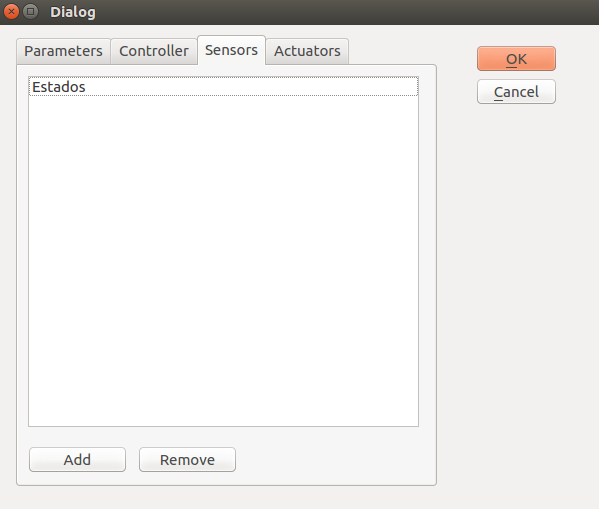
\includegraphics[width=230pt]{figuras/6.png}}
	\hfill
	\subfloat{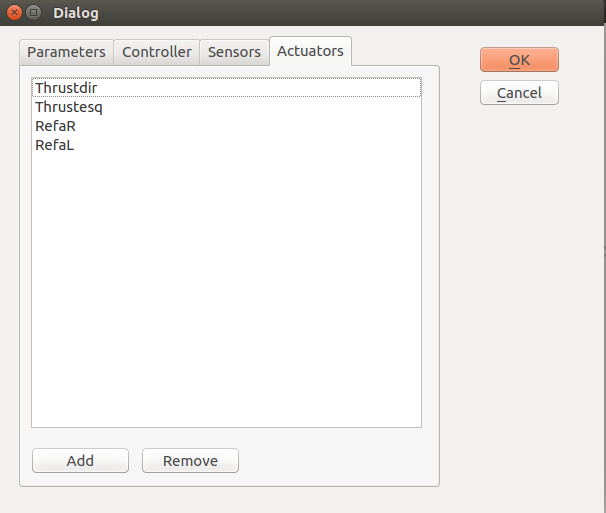
\includegraphics[width=230pt]{figuras/7.png}}
	\hfill
	\caption{Tabs \textit{Sensors} and \textit{Actuators}}
	\label{abas}
\end{figure}

In this example, the controller wil receive an array with scalar data containig information provided by a single sensor, whose communication topic is named \texttt{Estados}. The controller must return a floating point vector of size 4 with input control signals for the actuators, whose communication topics are in the following order:
\begin{enumerate}
\item \texttt{Thrustdir}
\item \texttt{Thrustesq}
\item \texttt{RefaR}
\item \texttt{RefaL}
\end{enumerate}

\subsection{Ceating a new control strategy}

To crate a new control strategy, press \textit{New Controller} in tab \textit{Controller}. A new window wil show up, requesting the user for the new controller's name. In this example, the control strategy will be called \texttt{vant2load\_hinfinity} (Figure \ref{projeto1}). After confirming the controller's name, a new Nautilus window will be opened with the directory for the created project (Figure \ref{2a}).

\begin{figure*}[!ht]
	\centering
	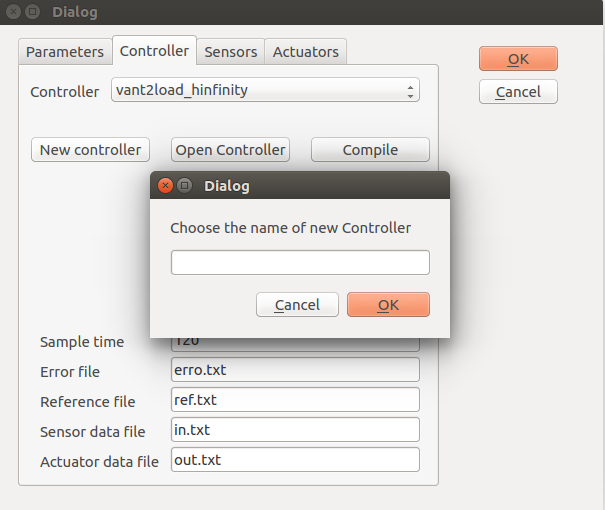
\includegraphics[width=0.7\columnwidth]{figuras/1a1a1.png}
	\caption{Ceating a new control strategy}
	\label{projeto1}
\end{figure*}

\begin{figure*}[!ht]
	\centering
	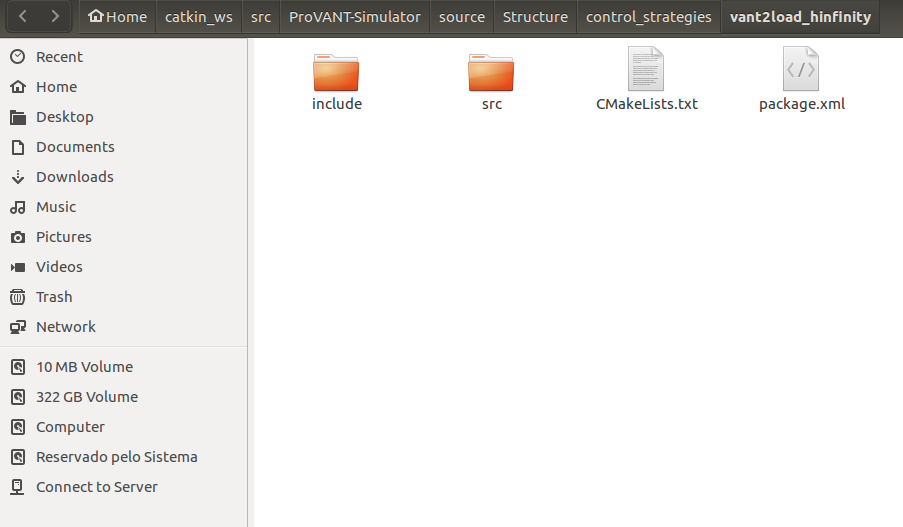
\includegraphics[width=0.7\columnwidth]{figuras/2a.png}
	\caption{Files and directories associated with the new control strategy}
	\label{2a}
\end{figure*}

\subsection{Implementing the new control strategy}

Code \ref{exemplo1} shows an example of control strategy code implemented in file \texttt{main.cpp}. It can be noted in the example that it is necessary to include three libraries:

%\begin{code}[H]
%\begin{minted}{cpp}
%#include "Icontroller.hpp"
%#include <Eigen/Eigen>
%#include "simulator_msgs/Sensor.h"
%	
%class hinfinity : public Icontroller 
%{
%	private: Eigen::VectorXd Xref; // vetor de referência
%	private: Eigen::VectorXd Erro; // vetor de erros
%	private: Eigen::VectorXd Input; // sinais de controle
%	private: Eigen::MatrixXd K; // matriz de ganhos do controlador
%	private: Eigen::VectorXd X; // vetor de estados
%	private: double T; // Período de amostragem
%	
%	public: hinfinity(): Xref(24), K(4,24), X(24), Erro(24), Input(4)
%	{ 
%		T = 0.012;
%	}
%	public: ~hinfinity(){	}
%	
%	public: void config()
%	{	
%		K<< [...] Dados da matriz [...];
%	}
%	public: std::vector<double> execute(simulator_msgs::SensorArray arraymsg)
%	{
%		static float count = 0;
%		static float xint, x_ant = 0;
%		static float yint, y_ant = 0;
%		static float zint, z_ant = 0;
%		static float yawint, yaw_ant = 0;
%		// selecionando dados
%		int i = 0;		
%		simulator_msgs::Sensor msgstates;
%		msgstates = arraymsg.values.at(0);
%\end{minted}	% Page break
%\end{code}
%\begin{code}[H]
%%begin{minted}{cpp}
%		// Referência
%		float trajectoryRadius = 2;
%		float trajectoryHeight = 4*trajectoryRadius;
%		float trajTime = 80;
%		float pi = 3.14;
%		float x = trajectoryRadius*cos((count*T)*2*pi/trajTime);
%		float xdot = -trajectoryRadius*(2*pi/trajTime)*sin((count*T)*2*pi/trajTime);
%		float xddot = -trajectoryRadius*(2*pi/trajTime)*(2*pi/trajTime)
%				*cos((count*T)*2*pi/trajTime);
%		float y = trajectoryRadius*sin((count*T)*2*pi/trajTime);
%		float ydot = trajectoryRadius*(2*pi/trajTime)*cos((count*T)*2*pi/trajTime);
%		float yddot = -trajectoryRadius*(2*pi/trajTime)*(2*pi/trajTime)
%				*sin((count*T)*2*pi/trajTime);
%		float z = trajectoryHeight+1 - trajectoryHeight*cos((count*T)*2*pi/trajTime);
%		float zdot = trajectoryHeight*(2*pi/trajTime)*sin((count*T)*2*pi/trajTime);
%		float zddot = trajectoryHeight*(2*pi/trajTime)*(2*pi/trajTime)
%				*cos((count*T)*2*pi/trajTime);
%		Xref << x,y,z,0,0,0,0.00002965,0.004885,0.004893,0.00484,xdot,ydot,zdot,
%			0,0,0,0,0,0,0,0,0,0,0;
%
%		//Convertendo velocidade angular
%		std::vector<double> etadot = pqr2EtaDot(msgstates.values.at(13),
%		msgstates.values.at(14),
%		msgstates.values.at(15),
%		msgstates.values.at(3),
%		msgstates.values.at(4),
%		msgstates.values.at(5));
%		
%		// Integrador Trapezoidal
%		float x_atual = msgstates.values.at(0) - Xref(0);
%		xint = xint + (T/2)*(x_atual + x_ant);
%		x_ant = x_atual;
%		float y_atual = msgstates.values.at(1) - Xref(1);
%		yint = yint + (T/2)*(y_atual + y_ant);
%		y_ant = y_atual;
%		float z_atual = msgstates.values.at(2) - Xref(2);
%		zint = zint + (T/2)*(z_atual + z_ant);
%		z_ant = z_atual;
%		float yaw_atual = msgstates.values.at(5) - Xref(5);
%		yawint = yawint + (T/2)*(yaw_atual + yaw_ant);
%		yaw_ant = yaw_atual;
%		
%		// vetor de estados aumentado
%		X << msgstates.values.at(0),//x
%		msgstates.values.at(1),//y
%		msgstates.values.at(2),//z
%		msgstates.values.at(3),//roll
%		msgstates.values.at(4),//pitch
%		msgstates.values.at(5),//yaw
%		msgstates.values.at(8),//g1 x
%		msgstates.values.at(9),//g2 y
%		msgstates.values.at(6),//aR
%		msgstates.values.at(7),//aL
%		msgstates.values.at(10),//vx
%		msgstates.values.at(11),//vy
%		msgstates.values.at(12),//vz
%\end{minted}	% Page break
%\end{code}
%\begin{code}[H]
%\begin{minted}{cpp}
%		etadot.at(0),//droll
%		etadot.at(1),//pitch
%		etadot.at(2),//yaw
%		msgstates.values.at(18),
%		msgstates.values.at(19),
%		msgstates.values.at(16),
%		msgstates.values.at(17),
%		xint,
%		yint,
%		zint,
%		yawint;
%		
		
%		// lei de controle
%		Erro = X-Xref;
%		Input = -K*Erro;
%		
%		Eigen::MatrixXd qref(10,1);
%		qref << x,y,z,0,0,0,0.00002965,0.004885,0.004893,0.00484;
%		Eigen::MatrixXd qrefdot(10,1);
%		qrefdot << xdot,ydot,zdot,0,0,0,0,0,0,0;
%		Eigen::MatrixXd qrefddot(10,1);
%		qrefddot << xddot,yddot,zddot,0,0,0,0,0,0,0;
%		Eigen::MatrixXd  varfeedforward  = feedforward::compute(qref,qrefdot,qrefddot);
%		
%		// Feedforward
%		Input(0) = Input(0) + 12.6005;
%		Input(1) = Input(1) + 12.609;
%		count++; 
%		
%		std::vector<float> out2(Input.data(), Input.data() + Input.rows() 
%					* Input.cols());
%		
%		std::vector<double> out(out2.size());
%		for(int i=0; i<out2.size();i++) out.at(i) = out2.at(i);
%		return out;
%	}
%	
%	public: std::vector<double> Reference()
%	{
%		std::vector<double> out(Xref.data(), Xref.data() + Xref.rows() 
%					* Xref.cols());
%		return out;
%	}
%	
%	public: std::vector<double> Error()
%	{
%		std::vector<double> out(Erro.data(), Erro.data() + Erro.rows() 
%					* Erro.cols());	
%		return out;
%	}	
%	
%	public: std::vector<double> State()
%	{
%		std::vector<double> out(X.data(), X.data() + X.rows() * X.cols());
%		return out;
%	}
%\end{minted}	% Page break
%\end{code}
\begin{code}[H]
\begin{minted}{cpp}
	private: std::vector<double> pqr2EtaDot(double in_a, double in_b, double in_c, 
						double phi, double theta, double psii)
	{
		std::vector<double> out;
		out.push_back(in_a + in_c*cos(phi)*tan(theta) + in_b*sin(phi)*tan(theta));
		out.push_back(in_b*cos(phi) - in_c*sin(phi));
		out.push_back((in_c*cos(phi))/cos(theta) + (in_b*sin(phi))/cos(theta));
		return out;
	}
};
	
extern "C"
{ 
	Icontroller *create(void) {
		return new hinfinity;
	}
	void destroy(Icontroller *p) {
		delete p;
	}
}
\end{minted}
\caption{Example code}
\label{exemplo1}
\end{code}

\begin{itemize}
		\setlength{\itemsep}{1pt}
		\setlength{\parskip}{0pt}
		\setlength{\parsep}{0pt}
\item \texttt{\#include ''Icontroller.hpp''} informs to the code the standard interface for creating controllers in the simulation environment;
\item \texttt{\#include <Eigen/Eigen>} imports the functionalities provided by library \texttt{Eigen}\footnote{https://eigen.tuxfamily.org}. This library provides funcitons for making linear algebra operations;
\item \texttt{\#include ''simulator\_msgs/Sensor.h''} informs the class responsible for the abstraction of the communication pattern between the controller and the sensors.
\end{itemize}

Attributes \texttt{Xref}, \texttt{Erro}, \texttt{Input}, \texttt{K} and \texttt{X} are \texttt{Eigen} library's vector and matrix structures, responsible for the linear algebra operation, thus allowing for the control strategy's execution. Atrtibute \texttt{T} determines the controller's sampling period.

Constructor \texttt{hinfinity()} inicializes the class' attibutes, while destructor \texttt{\textasciitilde hinfinity()} has no functionality in the simulator's context.

In this example, method \texttt{config()} is used to attribute values to the gain matrix \texttt K, respecting the \texttt{Eigen} library's sintax. However, the user can use this space to make any other initial configuration. Finally, the control strategy's logic is implemented in method \texttt{execute()}, that is executed at every sampling period, as previously mentioned.

The code begins declaring the (static) variable \texttt{xint}, \texttt{x\_ant}, \texttt{yint}, \texttt{y\_ant}, \texttt{zint}, \texttt{z\_ant}, \texttt{yawint} and \texttt{yaw\_ant}, used to store the values of the integrators impplemented in the contro lstrategy. Next comes the code piece regarding the sensors' data, obtained by vector \texttt{arraymsg}. Since only one sensor is available in this example (\texttt{Estados}), only the vector's first position is acessed (using the syntax \texttt{arraymsg.values.at(0)}). If more than one sensor were to be available, the n\textsuperscript{th} sensor's data would be accessed using \texttt{arraymsg.values.at(n-1)} and the order of this vector's elements would be defined in advance in tab \textit{Sensor}, as shown in \ref{6}. Next, the reference for the controller is defined and the integrators are implemented, using the trapezoidal integration method, for the realization of the control law. Finally, the feedfoward control action is calculated.

Methods \texttt{Reference()}, \texttt{Error()} and \texttt{State()} are used to store the reference, error and state signals, respectively, in the simulator's output text files. Function \texttt{pqr2EtaDot()} corresponds to a mapping of part of the information received by the sensors, required for this example's control strategy implementation.

Like function \texttt{pqr2EtaDot()}, any additional function required for the control strategy's implementation, which can also be related to filtering algorithms, can be written in \texttt{main.cpp}, or in auxiliary files created inside the folder \texttt{include/}, shown in \ref{2a} (in that case, they must also be included in \texttt{main.cpp}'s header).

Finally, the following code piece corresponds to the functions required to make sure the control strategy will be loaded in the simulator's execution time. Function \texttt{create()} creates an instance of the class that encapsulates the controller, and function \texttt{destroy()} is used to destruct the class's instance.

\begin{minted}{cpp}
extern "C"
{ 
	Icontroller *create(void) {
		return new hinfinity;
	}
	void destroy(Icontroller *p) {
		delete p;
	}
}
\end{minted}

\subsection{Compiling the control strategy's code}

After implementing the control strategy, the corresponding code can be compiled by pressing button \textit{Compile} (as explained in Chapter \ref{workflow}, see Figure \ref{5} item 4).